\documentclass{report}
\usepackage[spanish]{babel}



\usepackage[spanish]{babel}
\usepackage[utf8x]{inputenc}
\usepackage{amsmath}
\usepackage{graphicx}
\usepackage[colorinlistoftodos]{todonotes}
\usepackage{enumitem}
\usepackage{listings}
\usepackage{verbatim}
\usepackage{eurosym}
\usepackage[export]{adjustbox}
\usepackage{amssymb}
\usepackage{bussproofs}
\usepackage{amsmath}
\usepackage{tikz}
\usepackage{xcolor}
\usepackage{listings}
\usepackage{titletoc}
\usepackage{hyperref}

\hypersetup{
  colorlinks=true,
  linkcolor=black,
  urlcolor=blue,
  citecolor=black
}

\newcommand{\coverPage}[6]{%
%----------------------------------------------------------------------------------------
%	COVER START
%----------------------------------------------------------------------------------------
\begin{titlepage}

    \newcommand{\HRule}{\rule{\linewidth}{0.5mm}}
    \newcommand{\department}{#1}
    \newcommand{\course}{#2}
    \newcommand{\titleValue}{#3}
    \newcommand{\subtitleValue}{#4}
    \newcommand{\authorName}{#5}

    \center

    %----------------------------------------------------------------------------------------
    %	HEADER
    %----------------------------------------------------------------------------------------
    
\includegraphics{images/logo_usa.png}
    \vspace{0.5cm}
    \textsc{\Large \department}\\[0.5cm]
    \textsc{\Large \course}\\[0.5cm]
    \vfill

    %----------------------------------------------------------------------------------------
    %	TITLE
    %----------------------------------------------------------------------------------------

    \HRule\\
    \Huge
    \textbf{\titleValue}\\[0.5cm]
    \Large
    \textbf{\subtitleValue}\\
    \HRule\\[0.5cm]

    %----------------------------------------------------------------------------------------
    %	AUTHOR AND DATE
    %----------------------------------------------------------------------------------------

    \vfill
    \Large
    \textit{\authorName}\\
    {\large \today}\\[2cm]

\end{titlepage}
%----------------------------------------------------------------------------------------
%	COVER END
%----------------------------------------------------------------------------------------
}

\begin{document}
    \coverPage{ Matemáticas }{ Ecuaciones Diferenciales Ordinarias }{ Taller 7 }{  }{ Alexander Mendoza \\ Alejandro Garzón }{\today}

    \lstset{
        backgroundcolor=\color{white},   % background color for the code
        basicstyle=\footnotesize\ttfamily, % basic style of the code
        breaklines=true,                  % automatic line breaking
        frame=single,                     % adds a frame around the code
        numbers=left,                     % line numbers on the left
        numberstyle=\tiny\color{gray},    % style of the line numbers
        commentstyle=\color{green},       % style of comments
        keywordstyle=\color{blue},        % style of keywords
        stringstyle=\color{red}           % style of strings
    }

    \begin{lstlisting}[language=Python]
        import numpy as np
        import matplotlib.pyplot as plt
        
        
        def sistema_depredador_presa(Y):
            x, y = Y
            return np.array([2*x - 1.2*x*y, -y + 1.2*x*y])
        
        
        def resolver_sistema(Y0, dt, nt):
            Yt = np.zeros((2, nt+1))
            tt = np.zeros(nt+1)
            Yt[:, 0] = Y0
            t = 0
            Y = Y0.copy()
            for i in range(nt):
                Ym = Y + dt * sistema_depredador_presa(Y)
                Y = Y + dt / 2 * (sistema_depredador_presa(Y) + sistema_depredador_presa(Ym))
                t += dt
                Yt[:, i+1] = Y
                tt[i+1] = t
            return Yt, tt
        
        
        def funcion_lyapunov(x, y):
            return -1.2*x - np.log(x) + 1.2*y - 2*np.log(y)
        
        
        def grafica_evolucion_tiempo(tt, x, y):
            plt.figure(figsize=(8, 6))
            plt.plot(tt, x, linestyle='--', color='tab:red', label='x(t)', linewidth=2)
            plt.plot(tt, y, linestyle='-.', color='tab:blue', label='y(t)', linewidth=2)
            plt.legend(fontsize=12)
            plt.xlabel('$t$', fontsize=14)
            plt.ylabel('$x, y$', fontsize=14)
            plt.title('Grafica x(t) y(t)', fontsize=16)
            plt.grid(True, linestyle=':', color='gray', alpha=0.7)  # More subtle grid lines
            plt.tight_layout()
        
        
        def grafica_plano(x, y):
            plt.figure(figsize=(8, 6))
            plt.plot(x, y, linestyle='-', color='darkviolet', linewidth=2)
            plt.axis('equal')
            plt.xlabel('$x$', fontsize=14)
            plt.ylabel('$y$', fontsize=14)
            plt.title('Orbita', fontsize=16)
            plt.grid(True, linestyle=':', color='gray', alpha=0.7)
            plt.tight_layout()
        
        
        def grafica_plano_curva(x, y):
            xgrid = np.linspace(0.5, 3, 100)
            ygrid = np.linspace(0.5, 3, 100)
            X, Y = np.meshgrid(xgrid, ygrid)
            Z = funcion_lyapunov(X, Y)
        
            plt.figure(figsize=(8, 6))
            cp = plt.contour(X, Y, Z, levels=20, cmap='viridis')
            plt.plot(x, y, 'r-', linewidth=2)
            plt.colorbar(cp)
            plt.axis('equal')
            plt.xlabel('$x$', fontsize=14)
            plt.ylabel('$y$', fontsize=14)
            plt.title('Orbita con curva', fontsize=16)
            plt.grid(True, linestyle=':', color='gray', alpha=0.7)
            plt.legend(fontsize=12)
            plt.tight_layout()
        
        
        
        Y0 = np.array([1.75, 1.0])
        dt = 0.01
        nt = 1000
        
        Yt, tt = resolver_sistema(Y0, dt, nt)
        x, y = Yt[0, :], Yt[1, :]
        
        grafica_evolucion_tiempo(tt, x, y)
        grafica_plano(x, y)
        grafica_plano_curva(x, y)
        
        plt.show()
        
    \end{lstlisting}

    \begin{figure}[h!]
        \centering
        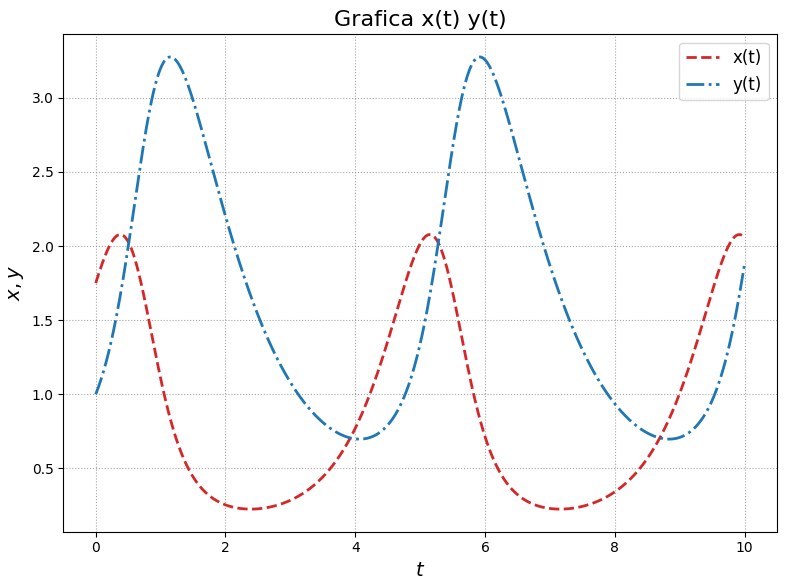
\includegraphics[width=0.8\textwidth]{images/image1.png}
      \end{figure}

      \begin{figure}[h!]
        \centering
        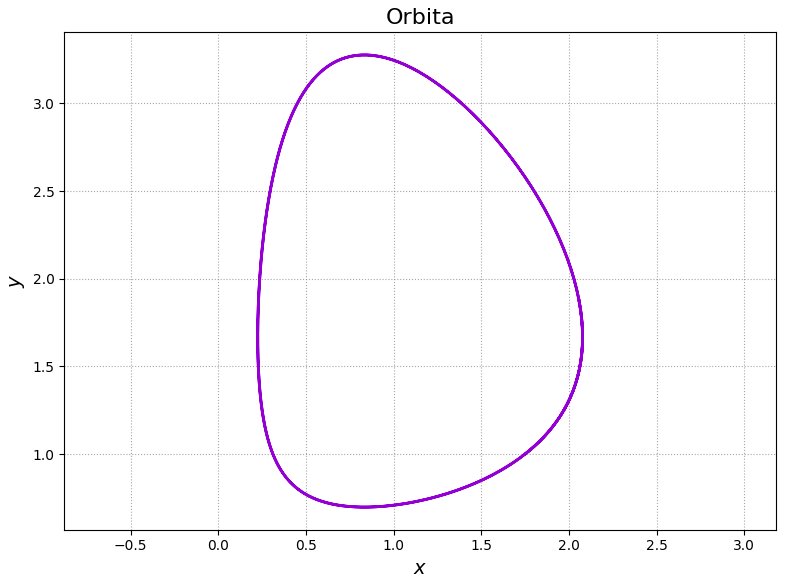
\includegraphics[width=0.8\textwidth]{images/image2.png}
      \end{figure}
      \begin{figure}[h!]
        \centering
        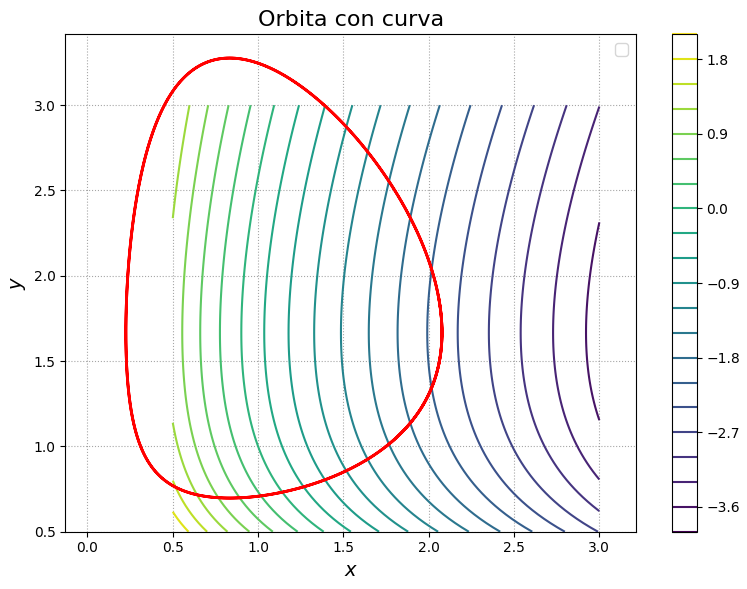
\includegraphics[width=0.8\textwidth]{images/image3.png}
      \end{figure}
\end{document}
